\section*{Глава 3. Разработка веб-приложения}
\addcontentsline{toc}{section}{Глава 3. Разработка веб-приложения}
\stepcounter{section}

В соответствии с результатами проектирования было разработано веб-приложение для ведения семейного бюджета.

\subsection{Вёрстка HTML страниц}

Разработка пользовательского интерфейса началась с создания базового шаблона \texttt{base.html}, который определяет общую структуру всех страниц приложения. Шаблон включает:
\begin{itemize}
    \item заголовок страницы с динамическим заголовком;
    \item подключение Bootstrap 5.3 (CSS и JS) через CDN;
    \item подключение кастомных стилей \texttt{style.css};
    \item навигационную панель (navbar), содержимое которой зависит от роли пользователя (owner, member, admin);
    \item блок для отображения flash-сообщений (уведомлений);
    \item основную область контента (блок \texttt{content});
    \item футер с копирайтом.
\end{itemize}

На основе базового шаблона были свёрстаны следующие страницы:
\begin{itemize}
    \item \texttt{auth/login.html} --- страница входа;
    \item \texttt{auth/register.html} --- страница регистрации (выбор роли: владелец/участник, поле email и кода семьи);
    \item \texttt{dashboard/owner\_dashboard.html} --- дашборд владельца семьи;
    \item \texttt{dashboard/member\_dashboard.html} --- дашборд участника семьи;
    \item \texttt{dashboard/admin\_dashboard.html} --- панель администратора;
    \item \texttt{dashboard/member\_stats.html} --- страница просмотра статистики участника (для владельца);
    \item \texttt{transactions.html} --- управление транзакциями с фильтрацией;
    \item \texttt{categories.html} --- управление категориями;
    \item \texttt{members.html} --- управление участниками семьи;
    \item \texttt{profile.html} --- страница профиля пользователя;
    \item \texttt{admin/all\_transactions.html} --- просмотр всех транзакций (админ);
    \item \texttt{admin/all\_files.html} --- просмотр всех загруженных файлов (админ).
\end{itemize}


\subsection{Реализация модуля авторизации}

Модуль авторизации реализован с использованием расширений \texttt{Flask-Login} (управление сессиями) и \texttt{bcrypt} (хэширование паролей) через методы \texttt{set\_password} и \texttt{check\_password} в модели \texttt{User}.

Регистрация пользователя реализована в маршруте \texttt{/auth/register} с учётом ролевой модели:
\begin{itemize}
    \item При выборе роли \textbf{«Владелец»} автоматически создаётся новая семья с названием «Семья \{username\}» и генерируется 6-значный код-приглашение (формата FAM-XXXXXX). Пользователь становится владельцем семьи. Также автоматически создаются 8 категорий по умолчанию: Продукты, Транспорт, Коммунальные услуги, Зарплата, Подработка, Кафе и рестораны, Развлечения, Одежда.
    \item При выборе роли \textbf{«Участник»} пользователь должен ввести код-приглашение существующей семьи. Система проверяет корректность кода и добавляет пользователя в соответствующую семью с ролью \texttt{'member'}.
\end{itemize}

Аутентификация выполняется через маршрут \texttt{/auth/login}. После успешного входа пользователь перенаправляется на дашборд, соответствующий его роли. Доступ к страницам контролируется декоратором \texttt{@login\_required}, а для разграничения прав используется проверка \texttt{current\_user.role}. Для администратора создана учётная запись по умолчанию (логин \texttt{'admin'}, пароль \texttt{'admin123'}), которая создаётся автоматически при инициализации базы данных.


\subsection{Реализация CRUD-интерфейса}

CRUD-интерфейс (Create, Read, Update, Delete) реализован для трёх основных сущностей: транзакции, категории и участники. Все операции выполняются через веб-формы с валидацией данных на стороне сервера.

\textbf{Управление транзакциями}

Для работы с транзакциями создана модель \texttt{Transaction}. Связь с чеком реализована через модель \texttt{Receipt}. Реализованы следующие маршруты и API-эндпоинты:
\begin{itemize}
    \item \texttt{GET /transactions} --- отображение списка транзакций с фильтрацией по поисковому запросу и диапазону дат;
    \item \texttt{POST /add\_transaction} --- добавление транзакции (сумма автоматически становится отрицательной для расходов);
    \item \texttt{POST /edit\_transaction} --- редактирование транзакции;
    \item \texttt{POST /api/delete\_transaction/<int:id>} --- удаление транзакции;
    \item \texttt{GET /api/get\_transaction/<int:id>} --- получение данных транзакции для редактирования.
\end{itemize}

При добавлении транзакции сумма вводится как положительное число, затем на основе типа категории определяется знак: для \texttt{'expense'} сумма становится отрицательной, для \texttt{'income'} --- положительной. Пользователь с ролью \texttt{'owner'} может добавлять транзакции для любого члена семьи, участник --- только для себя.

\textbf{Управление категориями}

Для реализации CRUD-функционала категорий создана модель \texttt{Category}. Категории доступны только для владельца семьи через маршрут \texttt{/categories}. Владелец может создавать, редактировать и удалять категории. При удалении категории все связанные с ней транзакции и чеки также удаляются для сохранения целостности данных.

Для установки лимитов на категории используется модель \texttt{CategoryLimit}. Установка лимита реализована через маршрут \texttt{/set\_category\_limit}. На странице категорий отображается текущий лимит для каждой категории (если установлен).

\textbf{Управление участниками}

Управление участниками семьи доступно владельцу через маршрут \texttt{/members}. На странице отображается список всех членов семьи с их ролями, email и установленным бюджетом. Реализованы следующие возможности:
\begin{itemize}
    \item \textbf{Просмотр} --- отображение всех участников с поиском по имени;
    \item \textbf{Установка бюджета} --- владелец может установить персональный бюджет для участника через маршрут \texttt{/set\_user\_budget} (модель \texttt{UserBudget});
    \item \textbf{Удаление участника} --- через API-эндпоинт \texttt{/api/delete\_member/<int:id>} (все транзакции и чеки участника также удаляются);
    \item \textbf{Генерация кода приглашения} --- через маршрут \texttt{/generate\_invite\_code}.
\end{itemize}

Все операции защищены проверкой роли: доступ только для \texttt{'owner'}.


\subsection{Реализация обработки и анализа данных}

Обработка и анализ данных реализованы на уровне маршрутов и моделей. В модели \texttt{User} добавлены методы \texttt{get\_transactions()}, \texttt{get\_total\_income()}, \texttt{get\_total\_expense()}, \texttt{get\_balance()}. Для оптимизации производительности используется модель \texttt{DashboardStats}, которая кэширует ежедневные балансы пользователей в поле \texttt{daily\_balance}. Функция \texttt{update\_dashboard\_stats(user\_id)} пересчитывает балансы после каждого изменения транзакций.

\textbf{Агрегация данных для дашбордов}

Для дашборда владельца семьи (\texttt{/dashboard/owner}) реализована следующая логика:
\begin{itemize}
    \item Расчёт общих доходов и расходов семьи за выбранный период (день/неделя/месяц);
    \item Расчёт семейного бюджета на основе суммы персональных бюджетов всех участников (с приведением к выбранному периоду);
    \item Группировка расходов по категориям для круговой диаграммы;
    \item Построение столбчатой диаграммы динамики баланса на основе кэшированных данных из \texttt{DashboardStats};
    \item Сводная таблица по участникам с доходами, расходами и балансом.
\end{itemize}

Для дашборда участника (\texttt{/dashboard/member}) реализована аналогичная логика, но только для одного пользователя. Владелец также может просматривать дашборд любого участника через маршрут \texttt{/member\_stats/<int:member\_id>}.

\textbf{Формирование отчётов}

Экспорт отчётов реализован в формате CSV через маршрут \texttt{/export\_report}. Отчёт включает все транзакции (для владельца --- всей семьи, для участника --- только свои) с колонками: дата, описание, категория, сумма, тип, участник. Файл автоматически скачивается с именем \texttt{report\_<period>\_<дата>.csv}.


\subsection{Реализация работы с файлами}

Модуль работы с файлами обеспечивает прикрепление чеков к транзакциям.

\textbf{Загрузка и хранение чеков}

При добавлении или редактировании транзакции пользователь может загрузить файл чека. Реализована следующая логика:
\begin{itemize}
    \item Допустимые форматы: изображения (.jpg, .jpeg, .png) и PDF;
    \item Максимальный размер файла: 16 МБ;
    \item Файл сохраняется в папке \texttt{uploads/} с использованием \texttt{secure\_filename};
    \item В таблице \texttt{Receipt} сохраняется путь к файлу и связь с транзакцией;
    \item При удалении транзакции связанный файл чека также удаляется с диска.
\end{itemize}

Просмотр чека реализован через API-эндпоинт \texttt{/api/get\_receipt/<int:id>}, который возвращает URL файла для отображения в модальном окне. Администратор имеет доступ к просмотру всех файлов через страницу \texttt{/admin/view\_all\_files}.


\subsection{Реализация системы визуализации}

Для наглядного отображения финансовой аналитики используется библиотека Chart.js. Визуализация реализована на дашбордах владельца и участника.

\textbf{Круговая диаграмма расходов по категориям}

Отображает структуру расходов за выбранный период. Данные передаются через переменные \texttt{expense\_categories} и \texttt{expense\_amounts}. Диаграмма строится с типом \texttt{pie} с цветовой палитрой из 10 цветов. При наведении на сектор отображается всплывающая подсказка с названием категории, суммой и процентным соотношением.

\begin{figure}[H]
    \centering
    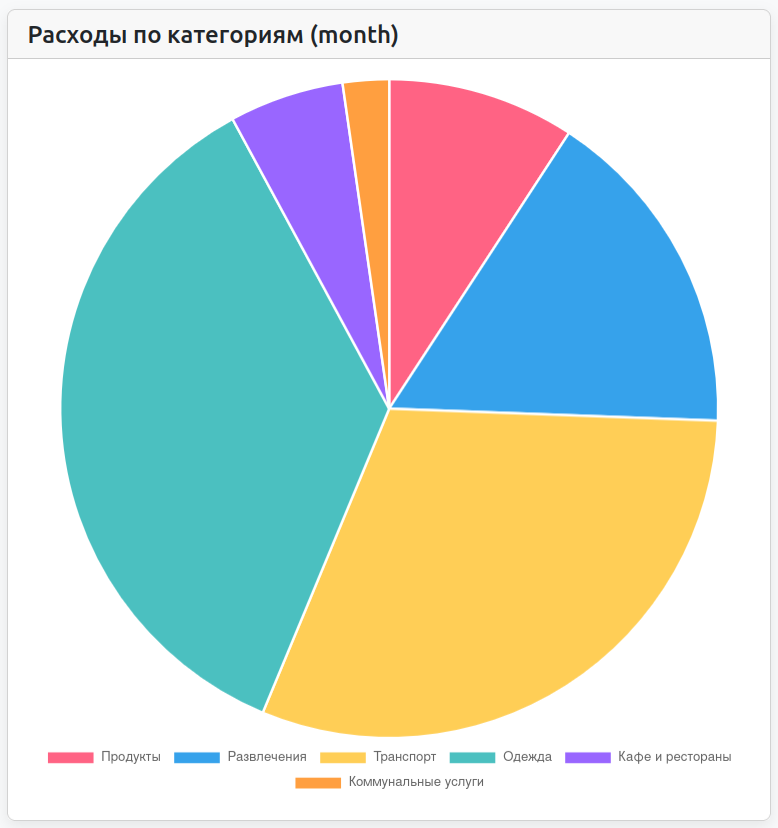
\includegraphics[width=0.7\textwidth]{images/pie_chart.png}
    \caption{Круговая диаграмма расходов по категориям}
    \label{fig:pie_chart}
\end{figure}

\textbf{Столбчатая диаграмма динамики баланса}

Показывает изменение баланса по дням выбранного периода. Данные передаются через переменные \texttt{chart\_labels} (метки дат) и \texttt{chart\_balance\_data} (значения баланса). Для владельца диаграмма имеет цветовое кодирование: зелёные столбцы для дней с положительным балансом, красные — для отрицательных, серые — для будущих дней. Диаграмма строится с типом \texttt{bar}.

\begin{figure}[H]
    \centering
    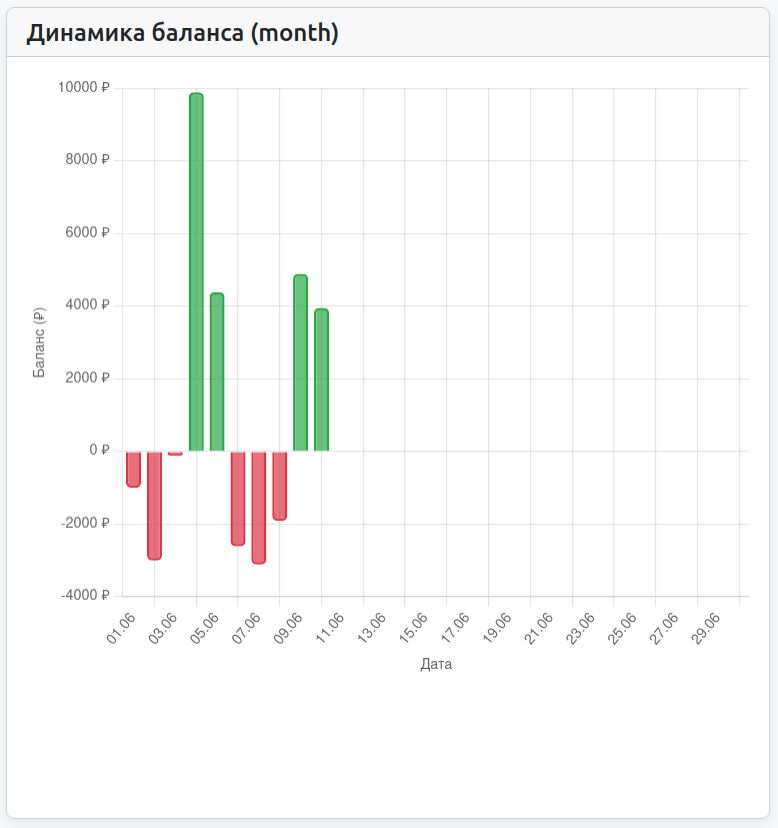
\includegraphics[width=0.7\textwidth]{images/bar_chart.png}
    \caption{Столбчатая диаграмма динамики баланса}
    \label{fig:bar_chart}
\end{figure}

\textbf{Сводная таблица по участникам}

На дашборде владельца реализована таблица с агрегированными данными по каждому участнику семьи: доходы, расходы, баланс. Для каждого участника предусмотрена кнопка «Дашборд», открывающая детальную статистику участника.

\begin{figure}[H]
    \centering
    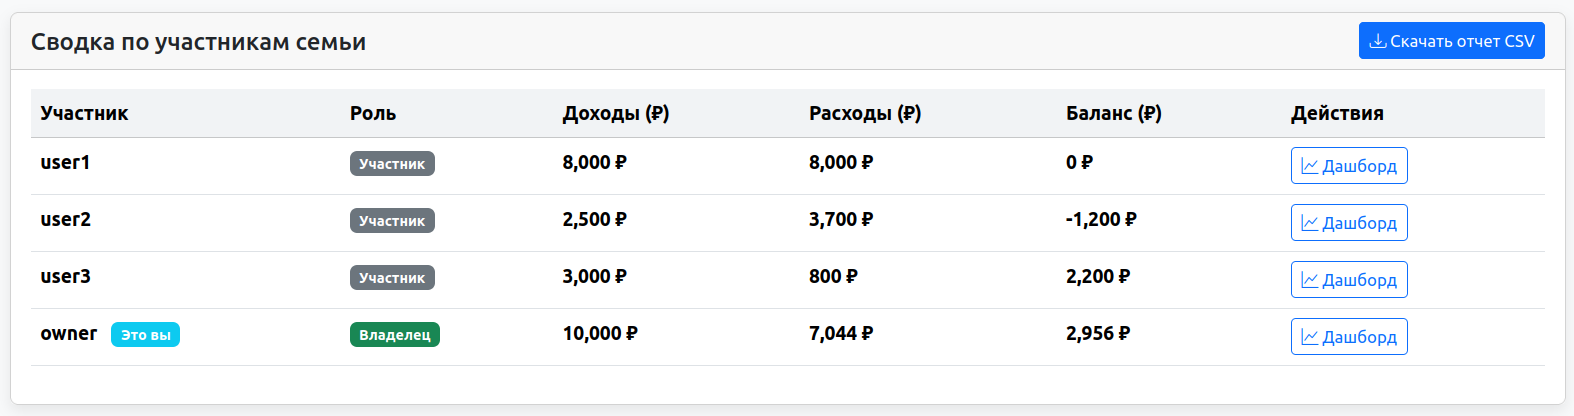
\includegraphics[width=0.9\textwidth]{images/members_table.png}
    \caption{Сводная таблица по участникам семьи}
    \label{fig:members_table}
\end{figure}

Все диаграммы автоматически перестраиваются при изменении периода через параметр URL \texttt{?period=}.
